%
% sa.tex
%
% (c) Roman Gassmann, HSR
%

\chapter{Simulated Annealing}
\rhead{Simulated Annealing}
\chapterauthor{Roman Gassmann}

Solange ein Optimierungsproblem gen"ugend einfach und von tiefer
Dimension ist, k"onnen optimalen Parameter mit
analytische Methoden gefunden werden.

Dies ist aber nicht mehr der Fall wenn die Komplexit"at und die Dimension
des Problems zu gross werden.
Kommt hinzu, dass in mehr-dimensionalen und komplexeren Problemen auch
h"aufig mehrere Minima/Maxima existieren. Es muss dann eine Reihe von
Tricks angewendet werden um ein einzelnes vern"unftiges/akzeptierbares
Minimum/Maximum zu finden.
	
\section{Local Search Method}
Wie bei allen Optimierungsproblemen gilt es die Zielfunktion
$f(\vec{x})$ zu minimieren. Dazu wird bei der lokalen Suchstrategie
in der Nachbarschaft $V(\vec{x}_n)$ von der L"osung $\vec{x}_n$
zuf"allig eine neue Parameterkombination
\[
\vec{x}_{n+1} =
V(\vec{x}_n) = \vec{x}_n + \vec{\gamma} \cdot v \qquad \text{mit }
\qquad
\begin{aligned}
\vec{\gamma}&= \text{Vektor mit Zufallsvariablen}\\
v& = \text{Umgebungsdistanz}
\end{aligned}
\]
gew"ahlt. Von dieser Kombination
wird der Funktionswert $f(\vec{x}_{n+1})$ berechnet. Ist dabei
\[
\Delta f = f(\vec{x}_{n+1}) - f(\vec{x}_{n})
\]
negativ, so wird
die Parameterkombination $\vec{x}_{n+1}$ als neue minimale L"osung
akzeptiert (Siehe Abb. \ref{localsearchsingle}). Ansonsten wird erneut
eine zuf"allige Kombination in der Nachbarschaft $V(\vec{x}_n)$ gew"ahlt.

\begin{figure}[ht!]
\usetikzlibrary{decorations.pathreplacing} 
\usetikzlibrary{calc}
\centering
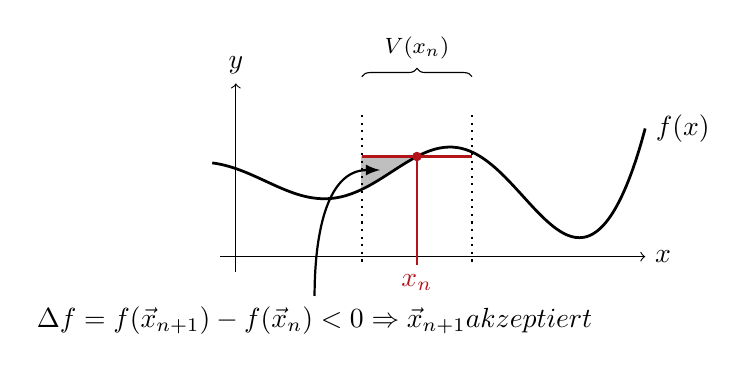
\begin{tikzpicture}[]%[>=latex']
\definecolor{CadetRed}		{cmyk}{0,1,1,0.290}
\def \v{0.7}


	\def\n{2.3}

	\coordinate (X) at (\n,0);
	\coordinate (XY) at (\n,{((5-\n)+1-1.3*sin(2*(5-\n)*180/pi))/((5-\n)+1)});
 %\shade[bottom color=lightgray, top color=white]  ($(-\v,0)+(XY)$) rectangle ($(\v,1)+(XY)$);
\filldraw[color=lightgray]  ($(-\v,0)+(XY)$) rectangle ($(\v,-0.5)+(XY)$);
\filldraw[smooth,samples=100,domain=-0.3:5.2, white, line width=1 ] (0,0.2)--plot (\x,{((5-\x)+1-1.3*sin(2*(5-\x)*180/pi))/((5-\x)+1)}) node[right] {$f(x)$} -- (5.2,0.2);
    \draw[->] (-0.2,0) -- (5.2,0)node[right] {$x$};
    \draw[->] (0,-0.2) -- (0,2.2) node[above] {$y$};
%\draw[cyan,dashed,line width=0.75] (-0.2,1.5)node[left]{$g+\varepsilon$} -- (5.2,1.5);
%\draw[blue,dashed, line width=0.75] (-0.2,1)node[left]{$g$} -- (5.2,1);
%\draw[cyan,dashed, line width=0.75] (-0.2,0.5)node[left]{$g-\varepsilon$} -- (5.2,0.5);

\draw[smooth,samples=100,domain=-0.3:5.2, black, line width=1 ] plot (\x,{((5-\x)+1-1.3*sin(2*(5-\x)*180/pi))/((5-\x)+1)}) node[right] {$f(x)$};

%\draw[smooth,samples=10,domain=\n-\v:\n, blue, line width=1 ] plot (\x,{((5-\x)+1-1.3*sin(2*(5-\x)*180/pi))/((5-\x)+1)});

\draw[CadetRed, line width=0.75] ($(-\v,0)+(XY)$ )--($(XY)+(\v,0)$);

\draw[CadetRed, line width=0.75] (XY) -- ($(X)+(0,-0.1)$)node[below]{$x_n$};
\draw[dotted, line width=0.75] ($(-\v,1.8)+(X)$) -- ($(-\v,-0.1)+(X)$);
\draw[dotted, line width=0.75] ($(X)+(\v,1.8)$) -- ($(X)+(\v,-0.1)$);
\filldraw[CadetRed] (XY) circle(1.5pt);

\draw [decorate,decoration={brace,amplitude=3pt,raise=1pt},yshift=0pt]
($(X)+(-\v,2.25)$) -- ($(X)+(\v,2.25)$) node [black,midway,yshift=0.4cm] {\footnotesize
$V(x_{n})$};

 \draw[-latex,thick](1,-0.5)node[below]
        {$\Delta f = f(\vec{x}_{n+1}) - f(\vec{x}_{n})< 0 \Rightarrow \vec{x}_{n+1} \text{ akzeptiert}$} to[out=90,in=180] (\n-2*\v/3,1.1);

\end{tikzpicture}
\caption{Lokale Suchstrategie}
\label{localsearchsingle}
\end{figure}

Dieser Vorgang wird nun eine bestimmte Anzahl mal oder solange bis keine
"Anderung mehr vorliegt durchgespielt.

Dabei ist klar, dass die Qualit"at der so gefunden L"osung sowohl
von der Startkombination $\vec{x}_0$, als auch von der Bestimmung der
Nachbarschaft $V(\vec{x})$ abh"angt. Gleichzeitig ist die Gefahr gross,
in einem lokalen Minimum der Zielfunktion h"angen zu bleiben (siehe
Abb. \ref{localsearch}).
\begin{figure}[ht!]
\usetikzlibrary{decorations.pathreplacing} 
\usetikzlibrary{calc}
\centering
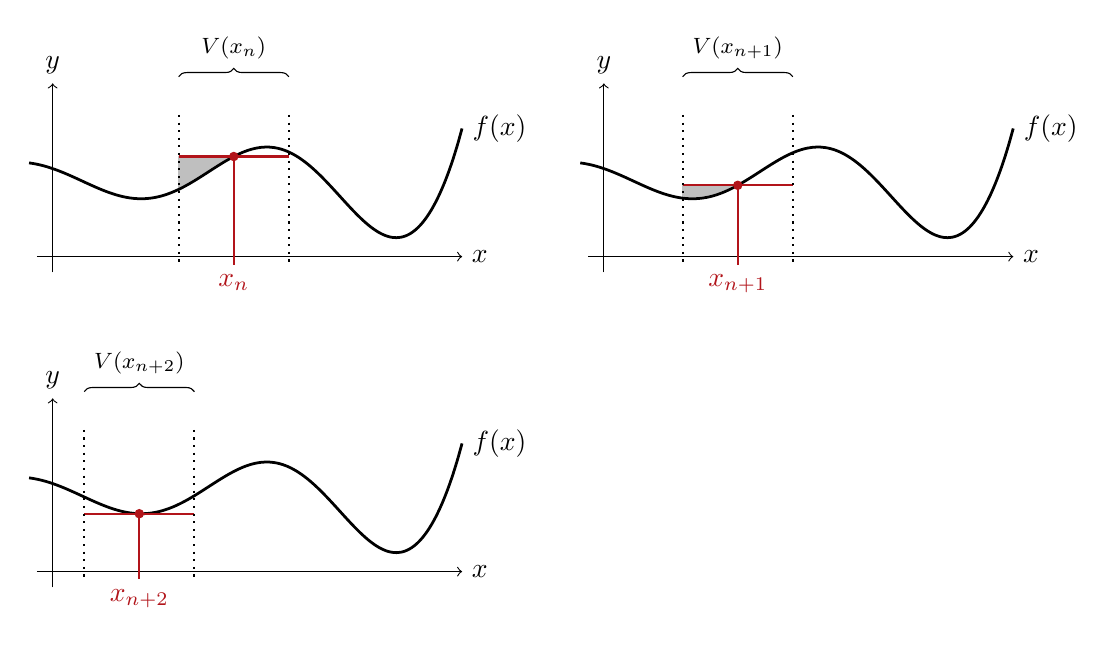
\begin{tikzpicture}[]%[>=latex']
\definecolor{CadetRed}		{cmyk}{0,1,1,0.290}
\def \v{0.7}

  %\draw[very thin,color=lightgray] (-0.5,-1.1) grid (5.2,2.2);
%\filldraw[gray!25] (0,0.5) rectangle (5.2,1.5);
\begin{scope}[]

	\def\n{2.3}

	\coordinate (X) at (\n,0);
	\coordinate (XY) at (\n,{((5-\n)+1-1.3*sin(2*(5-\n)*180/pi))/((5-\n)+1)});
 %\shade[bottom color=lightgray, top color=white]  ($(-\v,0)+(XY)$) rectangle ($(\v,1)+(XY)$);
\filldraw[color=lightgray]  ($(-\v,0)+(XY)$) rectangle ($(\v,-0.5)+(XY)$);
\filldraw[smooth,samples=100,domain=-0.3:5.2, white, line width=1 ] (0,0.2)--plot (\x,{((5-\x)+1-1.3*sin(2*(5-\x)*180/pi))/((5-\x)+1)}) node[right] {$f(x)$} -- (5.2,0.2);
    \draw[->] (-0.2,0) -- (5.2,0)node[right] {$x$};
    \draw[->] (0,-0.2) -- (0,2.2) node[above] {$y$};
%\draw[cyan,dashed,line width=0.75] (-0.2,1.5)node[left]{$g+\varepsilon$} -- (5.2,1.5);
%\draw[blue,dashed, line width=0.75] (-0.2,1)node[left]{$g$} -- (5.2,1);
%\draw[cyan,dashed, line width=0.75] (-0.2,0.5)node[left]{$g-\varepsilon$} -- (5.2,0.5);

\draw[smooth,samples=100,domain=-0.3:5.2, black, line width=1 ] plot (\x,{((5-\x)+1-1.3*sin(2*(5-\x)*180/pi))/((5-\x)+1)}) node[right] {$f(x)$};

\draw[CadetRed, line width=0.75] ($(-\v,0)+(XY)$ )--($(XY)+(\v,0)$);

\draw[CadetRed, line width=0.75] (XY) -- ($(X)+(0,-0.1)$)node[below]{$x_n$};
\draw[dotted, line width=0.75] ($(-\v,1.8)+(X)$) -- ($(-\v,-0.1)+(X)$);
\draw[dotted, line width=0.75] ($(X)+(\v,1.8)$) -- ($(X)+(\v,-0.1)$);
\filldraw[CadetRed] (XY) circle(1.5pt);

\draw [decorate,decoration={brace,amplitude=3pt,raise=1pt},yshift=0pt]
($(X)+(-\v,2.25)$) -- ($(X)+(\v,2.25)$) node [black,midway,yshift=0.4cm] {\footnotesize
$V(x_{n})$};


\end{scope}

\begin{scope}[xshift =7cm]
	\def\n{1.7}

	\coordinate (X) at (\n,0);
	\coordinate (XY) at (\n,{((5-\n)+1-1.3*sin(2*(5-\n)*180/pi))/((5-\n)+1)});
 %\shade[bottom color=lightgray, top color=white]  ($(-\v,0)+(XY)$) rectangle ($(\v,1)+(XY)$);
\filldraw[color=lightgray]  ($(-\v,0)+(XY)$) rectangle ($(\v,-0.9)+(XY)$);
\filldraw[smooth,samples=100,domain=-0.3:5.2, white, line width=1 ] (0,-0.5)--plot (\x,{((5-\x)+1-1.3*sin(2*(5-\x)*180/pi))/((5-\x)+1)})-- (5.2,-0.5);
    \draw[->] (-0.2,0) -- (5.2,0)node[right] {$x$};
    \draw[->] (0,-0.2) -- (0,2.2) node[above] {$y$};
%\draw[cyan,dashed,line width=0.75] (-0.2,1.5)node[left]{$g+\varepsilon$} -- (5.2,1.5);
%\draw[blue,dashed, line width=0.75] (-0.2,1)node[left]{$g$} -- (5.2,1);
%\draw[cyan,dashed, line width=0.75] (-0.2,0.5)node[left]{$g-\varepsilon$} -- (5.2,0.5);

\draw[smooth,samples=100,domain=-0.3:5.2, black, line width=1 ] plot (\x,{((5-\x)+1-1.3*sin(2*(5-\x)*180/pi))/((5-\x)+1)}) node[right] {$f(x)$};

\draw[CadetRed, line width=0.75] ($(-\v,0)+(XY)$ )--($(XY)+(\v,0)$);

\draw[CadetRed, line width=0.75] (XY) -- ($(X)+(0,-0.1)$)node[below]{$x_{n+1}$};
\draw[dotted, line width=0.75] ($(-\v,1.8)+(X)$) -- ($(-\v,-0.1)+(X)$);
\draw[dotted, line width=0.75] ($(X)+(\v,1.8)$) -- ($(X)+(\v,-0.1)$);
\filldraw[CadetRed] (XY) circle(1.5pt);

\draw [decorate,decoration={brace,amplitude=3pt,raise=1pt},yshift=0pt]
($(X)+(-\v,2.25)$) -- ($(X)+(\v,2.25)$) node [black,midway,yshift=0.4cm] {\footnotesize
$V(x_{n+1})$};
\end{scope}

\begin{scope}[yshift =-4cm]
	\def\n{1.1}

	\coordinate (X) at (\n,0);
	\coordinate (XY) at (\n,{((5-\n)+1-1.3*sin(2*(5-\n)*180/pi))/((5-\n)+1)});
 %\shade[bottom color=lightgray, top color=white]  ($(-\v,0)+(XY)$) rectangle ($(\v,1)+(XY)$);
\filldraw[color=lightgray]  ($(-\v,0)+(XY)$) rectangle ($(\v,-0.5)+(XY)$);
\filldraw[smooth,samples=100,domain=-0.3:5.2, white, line width=1 ] (0,-0.5)--plot (\x,{((5-\x)+1-1.3*sin(2*(5-\x)*180/pi))/((5-\x)+1)})-- (5.2,-0.5);
    \draw[->] (-0.2,0) -- (5.2,0)node[right] {$x$};
    \draw[->] (0,-0.2) -- (0,2.2) node[above] {$y$};

\draw[smooth,samples=100,domain=-0.3:5.2, black, line width=1 ] plot (\x,{((5-\x)+1-1.3*sin(2*(5-\x)*180/pi))/((5-\x)+1)}) node[right] {$f(x)$};

\draw[CadetRed, line width=0.75] ($(-\v,0)+(XY)$ )--($(XY)+(\v,0)$);

\draw[CadetRed, line width=0.75] (XY) -- ($(X)+(0,-0.1)$)node[below]{$x_{n+2}$};
\draw[dotted, line width=0.75] ($(-\v,1.8)+(X)$) -- ($(-\v,-0.1)+(X)$);
\draw[dotted, line width=0.75] ($(X)+(\v,1.8)$) -- ($(X)+(\v,-0.1)$);
\filldraw[CadetRed] (XY) circle(1.5pt);

\draw [decorate,decoration={brace,amplitude=3pt,raise=1pt},yshift=0pt]
($(X)+(-\v,2.25)$) -- ($(X)+(\v,2.25)$) node [black,midway,yshift=0.4cm] {\footnotesize
$V(x_{n+2})$};
\end{scope}

\end{tikzpicture}
\caption{Ablauf der lokalen Suchstrategie}
\label{localsearch}
\end{figure}
Es w"are also sinnvoll, tempor"ar auch schlechtere Parameterkombinationen zu zulassen, damit lokale Minima wieder verlassen werden k"onnen.

\section{Metropolis-Kriterium}
Nicholas Metropolis publizierte 1953 den Metropolisalgorithmus, welcher
\index{Metropolis, Nicolas}
\index{Metropolis-Kriterium}
sich genau diesem Problem annimmt. Er simuliert das Erreichen des
thermodynamischen Gleichgewichts eines Systems mit der Temperatur $T$.

Dabei wird wiederum wie bei der lokalen Suchstrategie
vorgegangen. Ausgehend von einem Punkt (Parameterkombination)
$\vec{x}_{n}$ wird in dessen Umgebung ein zuf"alliger Punkt
$\vec{x}_{n+1}$ gew"ahlt und
\[
\Delta f = f(\vec{x}_{n+1}) - f(\vec{x}_{n})
\]
berechnet.
Ist $\Delta f < 0$ wird mit $\vec{x}_{n+1}$ fortgefahren,
ist hingegen $\Delta f \geq 0$, wird $\vec{x}_{n+1}$
mit der Wahrscheinlichkeit
\[
p(\Delta f) = {\rm e}^{-\frac{\Delta f}{k_{\rm B} T}}\quad \text{mit }
\begin{aligned}k_{\rm B}&= \text{Bolzmann-Konstante}\\
T&= \text{Temperatur des Systems}
\end{aligned}
\]
trotzdem als neue L"osung akzeptiert.\\
\begin{figure}[ht!]
\centering
\usetikzlibrary{decorations.pathreplacing} 
\usetikzlibrary{calc}
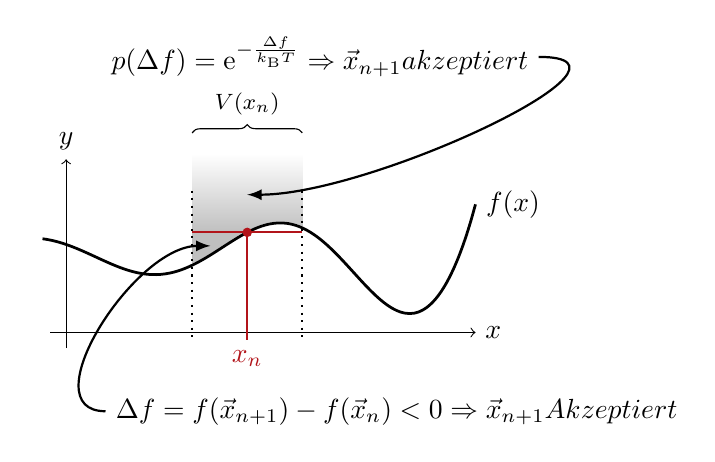
\begin{tikzpicture}[]%[>=latex']
\definecolor{CadetRed}		{cmyk}{0,1,1,0.290}
\def \v{0.7}


	\def\n{2.3}

	\coordinate (X) at (\n,0);
	\coordinate (XY) at (\n,{((5-\n)+1-1.3*sin(2*(5-\n)*180/pi))/((5-\n)+1)});
 \shade[bottom color=lightgray, top color=white]  ($(-\v,0)+(XY)$) rectangle ($(\v,1)+(XY)$);
\filldraw[color=lightgray]  ($(-\v,0)+(XY)$) rectangle ($(\v,-0.5)+(XY)$);
\filldraw[smooth,samples=100,domain=-0.3:5.2, white, line width=1 ] (0,0.2)--plot (\x,{((5-\x)+1-1.3*sin(2*(5-\x)*180/pi))/((5-\x)+1)}) node[right] {$f(x)$} -- (5.2,0.2);
    \draw[->] (-0.2,0) -- (5.2,0)node[right] {$x$};
    \draw[->] (0,-0.2) -- (0,2.2) node[above] {$y$};
%\draw[cyan,dashed,line width=0.75] (-0.2,1.5)node[left]{$g+\varepsilon$} -- (5.2,1.5);
%\draw[blue,dashed, line width=0.75] (-0.2,1)node[left]{$g$} -- (5.2,1);
%\draw[cyan,dashed, line width=0.75] (-0.2,0.5)node[left]{$g-\varepsilon$} -- (5.2,0.5);

\draw[smooth,samples=100,domain=-0.3:5.2, black, line width=1 ] plot (\x,{((5-\x)+1-1.3*sin(2*(5-\x)*180/pi))/((5-\x)+1)}) node[right] {$f(x)$};

\draw[CadetRed, line width=0.75] ($(-\v,0)+(XY)$ )--($(XY)+(\v,0)$);

\draw[CadetRed, line width=0.75] (XY) -- ($(X)+(0,-0.1)$)node[below]{$x_n$};
\draw[dotted, line width=0.75] ($(-\v,1.8)+(X)$) -- ($(-\v,-0.1)+(X)$);
\draw[dotted, line width=0.75] ($(X)+(\v,1.8)$) -- ($(X)+(\v,-0.1)$);
\filldraw[CadetRed] (XY) circle(1.5pt);

\draw [decorate,decoration={brace,amplitude=3pt,raise=1pt},yshift=0pt]
($(X)+(-\v,2.5)$) -- ($(X)+(\v,2.5)$) node [black,midway,yshift=0.4cm] {\footnotesize
$V(x_{n})$};

 \draw[-latex,thick](0.5,-1)node[right]
        {$\Delta f = f(\vec{x}_{n+1}) - f(\vec{x}_{n})< 0 \Rightarrow \vec{x}_{n+1} \text{ Akzeptiert}$} to[out=180,in=180] (\n-2*\v/3,1.1);

 \draw[-latex,thick](6,3.5)node[left]
        {$p(\Delta f ) = {\rm e}^{-\frac{\Delta f}{k_{\rm B} T}} \Rightarrow \vec{x}_{n+1} \text{ akzeptiert}$} to[out=0,in=0] (\n,1.75);

\end{tikzpicture}
\caption{Grafische Darstellung des Metropoliskriteriums}
\label{metropolissingle}
\end{figure}

Nicholas Metropolis bediente sich dabei der
Boltzmann-Statistik\footnote{Man erh"alt die Boltzmann-Statistik aus der
Annahme, dass alle Zust"ande im abgeschlossenen Gesamtsystem a priori
gleich wahrscheinlich sind. In den meisten F"allen wird der Einfachheit
halber $k_{\rm B} =1$ gesetzt} der Thermodynamik. Diese definiert die
Wahrscheinlichkeit $p(x)$ bei einer Temperatur $T$, den Zustand $x$
zu messen.
\begin{equation}p_x = {\rm e}^{-\frac{x}{k_{\rm B} T}}\label{Bolzmann}\end{equation}

Gem"ass der Formel \ref{Bolzmann} wird dem Optimierungsproblem also ein
\index{Bolzmann, Ludwig}
zus"atzlicher Paramater, der Temperaturparameter, hinzugef"ugt. Dieser
definiert die Temperatur des Systems/Problems. Je h"oher dabei die
Temperatur ist, desto h"oher ist die Wahrscheinlichkeit, dass eine
schlechtere Parameterkombination akzeptiert wird. Atomar betrachtet
heisst das, dass die einzelnen Atome (L"osungspunkte) des Systems sich
freier bewegen k"onnen.

Erst dadurch ist es also m"oglich lokale Minima wieder zu verlassen. Jedoch ist es mit konstanter Temperatur auch nicht mehr m"oglich eine konvergierende L"osung zu finden, da jedes Minimum wieder verlassen werden kann (siehe Abb. \ref{metropolis}).
\begin{figure}
\centering
\usetikzlibrary{decorations.pathreplacing} 
\usetikzlibrary{calc}
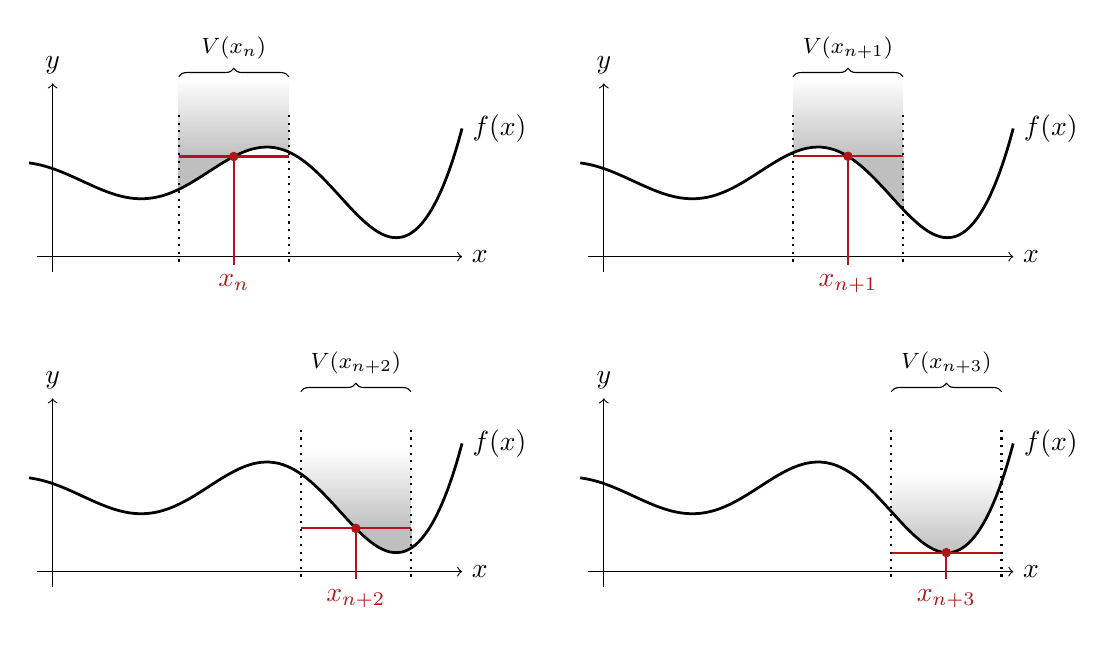
\begin{tikzpicture}[]%[>=latex']
\definecolor{CadetRed}		{cmyk}{0,1,1,0.290}
\def \v{0.7}

  %\draw[very thin,color=lightgray] (-0.5,-1.1) grid (5.2,2.2);
%\filldraw[gray!25] (0,0.5) rectangle (5.2,1.5);
\begin{scope}[]

	\def\n{2.3}

	\coordinate (X) at (\n,0);
	\coordinate (XY) at (\n,{((5-\n)+1-1.3*sin(2*(5-\n)*180/pi))/((5-\n)+1)});
 \shade[bottom color=lightgray, top color=white]  ($(-\v,0)+(XY)$) rectangle ($(\v,1)+(XY)$);
\filldraw[color=lightgray]  ($(-\v,0)+(XY)$) rectangle ($(\v,-0.5)+(XY)$);
\filldraw[smooth,samples=100,domain=-0.3:5.2, white, line width=1 ] (0,0.2)--plot (\x,{((5-\x)+1-1.3*sin(2*(5-\x)*180/pi))/((5-\x)+1)}) node[right] {$f(x)$} -- (5.2,0.2);
    \draw[->] (-0.2,0) -- (5.2,0)node[right] {$x$};
    \draw[->] (0,-0.2) -- (0,2.2) node[above] {$y$};
%\draw[cyan,dashed,line width=0.75] (-0.2,1.5)node[left]{$g+\varepsilon$} -- (5.2,1.5);
%\draw[blue,dashed, line width=0.75] (-0.2,1)node[left]{$g$} -- (5.2,1);
%\draw[cyan,dashed, line width=0.75] (-0.2,0.5)node[left]{$g-\varepsilon$} -- (5.2,0.5);

\draw[smooth,samples=100,domain=-0.3:5.2, black, line width=1 ] plot (\x,{((5-\x)+1-1.3*sin(2*(5-\x)*180/pi))/((5-\x)+1)}) node[right] {$f(x)$};

\draw[CadetRed, line width=0.75] ($(-\v,0)+(XY)$ )--($(XY)+(\v,0)$);

\draw[CadetRed, line width=0.75] (XY) -- ($(X)+(0,-0.1)$)node[below]{$x_n$};
\draw[dotted, line width=0.75] ($(-\v,1.8)+(X)$) -- ($(-\v,-0.1)+(X)$);
\draw[dotted, line width=0.75] ($(X)+(\v,1.8)$) -- ($(X)+(\v,-0.1)$);
\filldraw[CadetRed] (XY) circle(1.5pt);

\draw [decorate,decoration={brace,amplitude=3pt,raise=1pt},yshift=0pt]
($(X)+(-\v,2.25)$) -- ($(X)+(\v,2.25)$) node [black,midway,yshift=0.4cm] {\footnotesize
$V(x_{n})$};


\end{scope}

\begin{scope}[xshift =7cm]
	\def\n{3.1}

	\coordinate (X) at (\n,0);
	\coordinate (XY) at (\n,{((5-\n)+1-1.3*sin(2*(5-\n)*180/pi))/((5-\n)+1)});
 \shade[bottom color=lightgray, top color=white]  ($(-\v,0)+(XY)$) rectangle ($(\v,1)+(XY)$);
\filldraw[color=lightgray]  ($(-\v,0)+(XY)$) rectangle ($(\v,-0.9)+(XY)$);
\filldraw[smooth,samples=100,domain=-0.3:5.2, white, line width=1 ] (0,-0.5)--plot (\x,{((5-\x)+1-1.3*sin(2*(5-\x)*180/pi))/((5-\x)+1)})-- (5.2,-0.5);
    \draw[->] (-0.2,0) -- (5.2,0)node[right] {$x$};
    \draw[->] (0,-0.2) -- (0,2.2) node[above] {$y$};
%\draw[cyan,dashed,line width=0.75] (-0.2,1.5)node[left]{$g+\varepsilon$} -- (5.2,1.5);
%\draw[blue,dashed, line width=0.75] (-0.2,1)node[left]{$g$} -- (5.2,1);
%\draw[cyan,dashed, line width=0.75] (-0.2,0.5)node[left]{$g-\varepsilon$} -- (5.2,0.5);

\draw[smooth,samples=100,domain=-0.3:5.2, black, line width=1 ] plot (\x,{((5-\x)+1-1.3*sin(2*(5-\x)*180/pi))/((5-\x)+1)}) node[right] {$f(x)$};

\draw[CadetRed, line width=0.75] ($(-\v,0)+(XY)$ )--($(XY)+(\v,0)$);

\draw[CadetRed, line width=0.75] (XY) -- ($(X)+(0,-0.1)$)node[below]{$x_{n+1}$};
\draw[dotted, line width=0.75] ($(-\v,1.8)+(X)$) -- ($(-\v,-0.1)+(X)$);
\draw[dotted, line width=0.75] ($(X)+(\v,1.8)$) -- ($(X)+(\v,-0.1)$);
\filldraw[CadetRed] (XY) circle(1.5pt);

\draw [decorate,decoration={brace,amplitude=3pt,raise=1pt},yshift=0pt]
($(X)+(-\v,2.25)$) -- ($(X)+(\v,2.25)$) node [black,midway,yshift=0.4cm] {\footnotesize
$V(x_{n+1})$};
\end{scope}

\begin{scope}[yshift =-4cm]
	\def\n{3.85}

	\coordinate (X) at (\n,0);
	\coordinate (XY) at (\n,{((5-\n)+1-1.3*sin(2*(5-\n)*180/pi))/((5-\n)+1)});
 \shade[bottom color=lightgray, top color=white]  ($(-\v,0)+(XY)$) rectangle ($(\v,1)+(XY)$);
\filldraw[color=lightgray]  ($(-\v,0)+(XY)$) rectangle ($(\v,-0.5)+(XY)$);
\filldraw[smooth,samples=100,domain=-0.3:5.2, white, line width=1 ] (0,-0.5)--plot (\x,{((5-\x)+1-1.3*sin(2*(5-\x)*180/pi))/((5-\x)+1)})-- (5.2,-0.5);
    \draw[->] (-0.2,0) -- (5.2,0)node[right] {$x$};
    \draw[->] (0,-0.2) -- (0,2.2) node[above] {$y$};

\draw[smooth,samples=100,domain=-0.3:5.2, black, line width=1 ] plot (\x,{((5-\x)+1-1.3*sin(2*(5-\x)*180/pi))/((5-\x)+1)}) node[right] {$f(x)$};

\draw[CadetRed, line width=0.75] ($(-\v,0)+(XY)$ )--($(XY)+(\v,0)$);

\draw[CadetRed, line width=0.75] (XY) -- ($(X)+(0,-0.1)$)node[below]{$x_{n+2}$};
\draw[dotted, line width=0.75] ($(-\v,1.8)+(X)$) -- ($(-\v,-0.1)+(X)$);
\draw[dotted, line width=0.75] ($(X)+(\v,1.8)$) -- ($(X)+(\v,-0.1)$);
\filldraw[CadetRed] (XY) circle(1.5pt);

\draw [decorate,decoration={brace,amplitude=3pt,raise=1pt},yshift=0pt]
($(X)+(-\v,2.25)$) -- ($(X)+(\v,2.25)$) node [black,midway,yshift=0.4cm] {\footnotesize
$V(x_{n+2})$};
\end{scope}

\begin{scope}[yshift =-4cm, xshift =7cm]
	\def\n{4.35}

	\coordinate (X) at (\n,0);
	\coordinate (XY) at (\n,{((5-\n)+1-1.3*sin(2*(5-\n)*180/pi))/((5-\n)+1)});
 \shade[bottom color=lightgray, top color=white]  ($(-\v,0)+(XY)$) rectangle ($(\v,1)+(XY)$);
\filldraw[color=lightgray]  ($(-\v,0)+(XY)$) rectangle ($(\v,-0.5)+(XY)$);
\filldraw[smooth,samples=100,domain=-0.3:5.2, white, line width=1 ] (0,-0.5)--plot (\x,{((5-\x)+1-1.3*sin(2*(5-\x)*180/pi))/((5-\x)+1)})-- (5.2,-0.5);
    \draw[->] (-0.2,0) -- (5.2,0)node[right] {$x$};
    \draw[->] (0,-0.2) -- (0,2.2) node[above] {$y$};

\draw[smooth,samples=100,domain=-0.3:5.2, black, line width=1 ] plot (\x,{((5-\x)+1-1.3*sin(2*(5-\x)*180/pi))/((5-\x)+1)}) node[right] {$f(x)$};

\draw[CadetRed, line width=0.75] ($(-\v,0)+(XY)$ )--($(XY)+(\v,0)$);

\draw[CadetRed, line width=0.75] (XY) -- ($(X)+(0,-0.1)$)node[below]{$x_{n+3}$};
\draw[dotted, line width=0.75] ($(-\v,1.8)+(X)$) -- ($(-\v,-0.1)+(X)$);
\draw[dotted, line width=0.75] ($(X)+(\v,1.8)$) -- ($(X)+(\v,-0.1)$);
\filldraw[CadetRed] (XY) circle(1.5pt);

\draw [decorate,decoration={brace,amplitude=3pt,raise=1pt},yshift=0pt]
($(X)+(-\v,2.25)$) -- ($(X)+(\v,2.25)$) node [black,midway,yshift=0.4cm] {\footnotesize
$V(x_{n+3})$};
\end{scope}

\end{tikzpicture}
\caption{Grafischer Ablauf des Metropolisalgorithmus}
\label{metropolis}
\end{figure}
Es ist daher zwingend notwendig den Temperaturparameter zu kontrollieren.

\section{Simulated Annealing}
	Wird beim Metropolisalgorithmus mit einer hohen Temperatur begonnen (damit m"oglichst das gesammte System abgesucht wird) und anschliessend die Temperatur langsam abgesenkt, wird es immer wahrscheinlicher, dass man sich dem Minimum ann"ahert (Siehe Abb. \ref{siman}). Ist dabei die Temperatur von der Simulationszeit abh"angig, wird dieser Algorithmus als simulierte Abk"uhlung (Simulated Annealing) bezeichnet. %(Anzahl Durchl"aufe bei konstanter Temperatur)
\begin{figure}[ht!]
\centering
\usetikzlibrary{decorations.pathreplacing} 
\usetikzlibrary{calc}
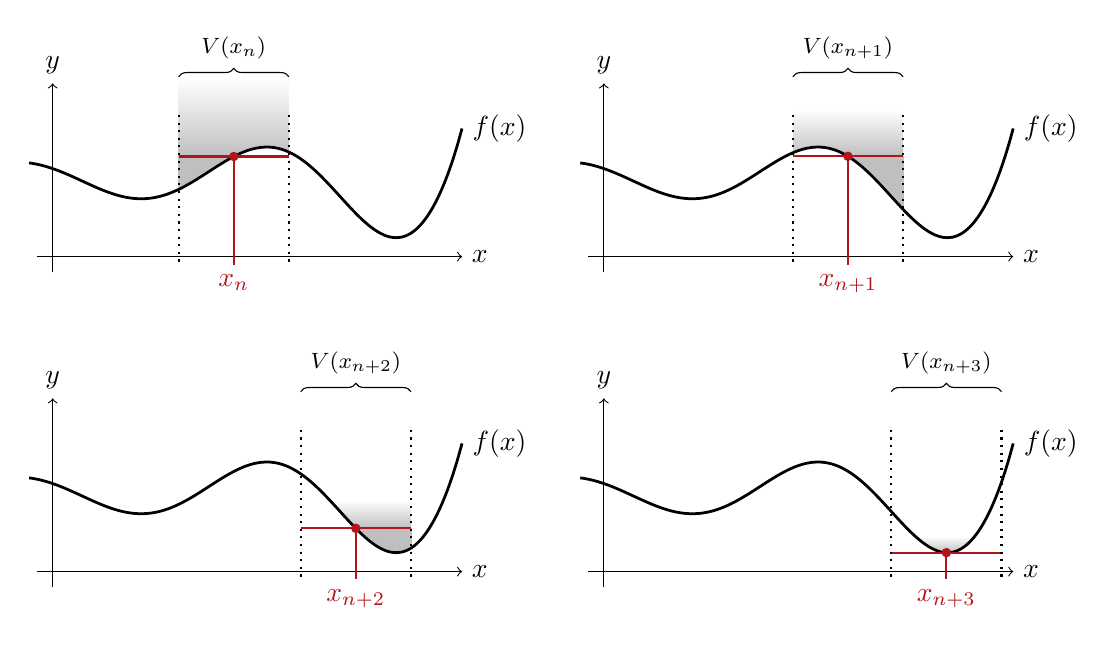
\begin{tikzpicture}[]%[>=latex']
\definecolor{CadetRed}		{cmyk}{0,1,1,0.290}
\def \v{0.7}

  %\draw[very thin,color=lightgray] (-0.5,-1.1) grid (5.2,2.2);
%\filldraw[gray!25] (0,0.5) rectangle (5.2,1.5);
\begin{scope}[]

	\def\n{2.3}

	\coordinate (X) at (\n,0);
	\coordinate (XY) at (\n,{((5-\n)+1-1.3*sin(2*(5-\n)*180/pi))/((5-\n)+1)});
 \shade[bottom color=lightgray, top color=white]  ($(-\v,0)+(XY)$) rectangle ($(\v,1)+(XY)$);
\filldraw[color=lightgray]  ($(-\v,0)+(XY)$) rectangle ($(\v,-0.5)+(XY)$);
\filldraw[smooth,samples=100,domain=-0.3:5.2, white, line width=1 ] (0,0.2)--plot (\x,{((5-\x)+1-1.3*sin(2*(5-\x)*180/pi))/((5-\x)+1)}) node[right] {$f(x)$} -- (5.2,0.2);
    \draw[->] (-0.2,0) -- (5.2,0)node[right] {$x$};
    \draw[->] (0,-0.2) -- (0,2.2) node[above] {$y$};
%\draw[cyan,dashed,line width=0.75] (-0.2,1.5)node[left]{$g+\varepsilon$} -- (5.2,1.5);
%\draw[blue,dashed, line width=0.75] (-0.2,1)node[left]{$g$} -- (5.2,1);
%\draw[cyan,dashed, line width=0.75] (-0.2,0.5)node[left]{$g-\varepsilon$} -- (5.2,0.5);

\draw[smooth,samples=100,domain=-0.3:5.2, black, line width=1 ] plot (\x,{((5-\x)+1-1.3*sin(2*(5-\x)*180/pi))/((5-\x)+1)}) node[right] {$f(x)$};

\draw[CadetRed, line width=0.75] ($(-\v,0)+(XY)$ )--($(XY)+(\v,0)$);

\draw[CadetRed, line width=0.75] (XY) -- ($(X)+(0,-0.1)$)node[below]{$x_n$};
\draw[dotted, line width=0.75] ($(-\v,1.8)+(X)$) -- ($(-\v,-0.1)+(X)$);
\draw[dotted, line width=0.75] ($(X)+(\v,1.8)$) -- ($(X)+(\v,-0.1)$);
\filldraw[CadetRed] (XY) circle(1.5pt);

\draw [decorate,decoration={brace,amplitude=3pt,raise=1pt},yshift=0pt]
($(X)+(-\v,2.25)$) -- ($(X)+(\v,2.25)$) node [black,midway,yshift=0.4cm] {\footnotesize
$V(x_{n})$};


\end{scope}

\begin{scope}[xshift =7cm]
	\def\n{3.1}

	\coordinate (X) at (\n,0);
	\coordinate (XY) at (\n,{((5-\n)+1-1.3*sin(2*(5-\n)*180/pi))/((5-\n)+1)});
 \shade[bottom color=lightgray, top color=white]  ($(-\v,0)+(XY)$) rectangle ($(\v,0.6)+(XY)$);
\filldraw[color=lightgray]  ($(-\v,0)+(XY)$) rectangle ($(\v,-0.9)+(XY)$);
\filldraw[smooth,samples=100,domain=-0.3:5.2, white, line width=1 ] (0,-0.5)--plot (\x,{((5-\x)+1-1.3*sin(2*(5-\x)*180/pi))/((5-\x)+1)})-- (5.2,-0.5);
    \draw[->] (-0.2,0) -- (5.2,0)node[right] {$x$};
    \draw[->] (0,-0.2) -- (0,2.2) node[above] {$y$};
%\draw[cyan,dashed,line width=0.75] (-0.2,1.5)node[left]{$g+\varepsilon$} -- (5.2,1.5);
%\draw[blue,dashed, line width=0.75] (-0.2,1)node[left]{$g$} -- (5.2,1);
%\draw[cyan,dashed, line width=0.75] (-0.2,0.5)node[left]{$g-\varepsilon$} -- (5.2,0.5);

\draw[smooth,samples=100,domain=-0.3:5.2, black, line width=1 ] plot (\x,{((5-\x)+1-1.3*sin(2*(5-\x)*180/pi))/((5-\x)+1)}) node[right] {$f(x)$};

\draw[CadetRed, line width=0.75] ($(-\v,0)+(XY)$ )--($(XY)+(\v,0)$);

\draw[CadetRed, line width=0.75] (XY) -- ($(X)+(0,-0.1)$)node[below]{$x_{n+1}$};
\draw[dotted, line width=0.75] ($(-\v,1.8)+(X)$) -- ($(-\v,-0.1)+(X)$);
\draw[dotted, line width=0.75] ($(X)+(\v,1.8)$) -- ($(X)+(\v,-0.1)$);
\filldraw[CadetRed] (XY) circle(1.5pt);

\draw [decorate,decoration={brace,amplitude=3pt,raise=1pt},yshift=0pt]
($(X)+(-\v,2.25)$) -- ($(X)+(\v,2.25)$) node [black,midway,yshift=0.4cm] {\footnotesize
$V(x_{n+1})$};
\end{scope}

\begin{scope}[yshift =-4cm]
	\def\n{3.85}

	\coordinate (X) at (\n,0);
	\coordinate (XY) at (\n,{((5-\n)+1-1.3*sin(2*(5-\n)*180/pi))/((5-\n)+1)});
 \shade[bottom color=lightgray, top color=white]  ($(-\v,0)+(XY)$) rectangle ($(\v,0.36)+(XY)$);
\filldraw[color=lightgray]  ($(-\v,0)+(XY)$) rectangle ($(\v,-0.5)+(XY)$);
\filldraw[smooth,samples=100,domain=-0.3:5.2, white, line width=1 ] (0,-0.5)--plot (\x,{((5-\x)+1-1.3*sin(2*(5-\x)*180/pi))/((5-\x)+1)})-- (5.2,-0.5);
    \draw[->] (-0.2,0) -- (5.2,0)node[right] {$x$};
    \draw[->] (0,-0.2) -- (0,2.2) node[above] {$y$};

\draw[smooth,samples=100,domain=-0.3:5.2, black, line width=1 ] plot (\x,{((5-\x)+1-1.3*sin(2*(5-\x)*180/pi))/((5-\x)+1)}) node[right] {$f(x)$};

\draw[CadetRed, line width=0.75] ($(-\v,0)+(XY)$ )--($(XY)+(\v,0)$);

\draw[CadetRed, line width=0.75] (XY) -- ($(X)+(0,-0.1)$)node[below]{$x_{n+2}$};
\draw[dotted, line width=0.75] ($(-\v,1.8)+(X)$) -- ($(-\v,-0.1)+(X)$);
\draw[dotted, line width=0.75] ($(X)+(\v,1.8)$) -- ($(X)+(\v,-0.1)$);
\filldraw[CadetRed] (XY) circle(1.5pt);

\draw [decorate,decoration={brace,amplitude=3pt,raise=1pt},yshift=0pt]
($(X)+(-\v,2.25)$) -- ($(X)+(\v,2.25)$) node [black,midway,yshift=0.4cm] {\footnotesize
$V(x_{n+2})$};
\end{scope}

\begin{scope}[yshift =-4cm, xshift =7cm]
	\def\n{4.35}

	\coordinate (X) at (\n,0);
	\coordinate (XY) at (\n,{((5-\n)+1-1.3*sin(2*(5-\n)*180/pi))/((5-\n)+1)});
 \shade[bottom color=lightgray, top color=white]  ($(-\v,0)+(XY)$) rectangle ($(\v,0.21)+(XY)$);
\filldraw[color=lightgray]  ($(-\v,0)+(XY)$) rectangle ($(\v,-0.5)+(XY)$);
\filldraw[smooth,samples=100,domain=-0.3:5.2, white, line width=1 ] (0,-0.5)--plot (\x,{((5-\x)+1-1.3*sin(2*(5-\x)*180/pi))/((5-\x)+1)})-- (5.2,-0.5);
    \draw[->] (-0.2,0) -- (5.2,0)node[right] {$x$};
    \draw[->] (0,-0.2) -- (0,2.2) node[above] {$y$};

\draw[smooth,samples=100,domain=-0.3:5.2, black, line width=1 ] plot (\x,{((5-\x)+1-1.3*sin(2*(5-\x)*180/pi))/((5-\x)+1)}) node[right] {$f(x)$};

\draw[CadetRed, line width=0.75] ($(-\v,0)+(XY)$ )--($(XY)+(\v,0)$);

\draw[CadetRed, line width=0.75] (XY) -- ($(X)+(0,-0.1)$)node[below]{$x_{n+3}$};
\draw[dotted, line width=0.75] ($(-\v,1.8)+(X)$) -- ($(-\v,-0.1)+(X)$);
\draw[dotted, line width=0.75] ($(X)+(\v,1.8)$) -- ($(X)+(\v,-0.1)$);
\filldraw[CadetRed] (XY) circle(1.5pt);

\draw [decorate,decoration={brace,amplitude=3pt,raise=1pt},yshift=0pt]
($(X)+(-\v,2.25)$) -- ($(X)+(\v,2.25)$) node [black,midway,yshift=0.4cm] {\footnotesize
$V(x_{n+3})$};
\end{scope}

\end{tikzpicture}
\caption{Grafischer Ablauf einer simulierten Abk"uhlung}
\label{siman}
\end{figure}
Um die Abk"uhlung zu simulieren wird folglich ein weiterer Parameter der Temperaturkoeffizient eingef"uhrt, welcher die Temperatur schrittweise verringert. Dabei w"are es w"unschenswert, dass bei einer bestimmten Temperatur mehrere Durchl"aufegemacht werden, um das Systemgebiet m"oglichst vollst"andig abzusuchen. Aus diesem Grund wird zus"atzlich der Iterationsparameter eingef"ugt, welcher daf"ur sorgt, dass die Temperatur nicht zu schnell verringert wird.

\subsection{Wahl der einzelnen Parameter}
\begin{description}
\item [Temperatur $T$] $ $\\
Grunds"atzlich kann f"ur ein beliebiges Optimierungsproblem als
Initial-Tem\-pe\-ratur der Durchschnitt einer Anzahl von zuf"alligen
Funktionswerten der Zielfunktion verwendet werden.
\item [Temperatur Koeffizient $c$] $ $\\
Um die Temperatur beeinflussen zu k"onnen wird der Temperaturkoeffizient
eingef"uhrt. Dieser ist typischerweise zwischen 0.6 und 0.9.

\item [Iterationsschritte bei konstanter Temperatur]$ $\\
Definiert die Anzahl Itterationen bevor die Temperatur verringert wird.
Typischer Wert im Bereich 50-100.

\item [Umgebungsdistanz $v$]$ $\\
Die Umgebungsdistanz $v$ definiert das Gebiet um $\vec{x}_{n}$,
in dem das n"achste Parameterset $\vec{x}_{n+1}$ gew"ahlt wird.
Dieser Parameter ist stark von der Zielfunktion abh"angig.
\end{description}
		
\clearpage
%\subsection{Pseudocode}

%\begin{lstlisting}[frame=none]
%	Init Startparameterset x[0]
%	loops = 1
%	i = 1
%	do{
%		generate x[i]= x[i-1] + uv
%		if( f(x[i]) < f(x[i-1]) ){
%			accept x[i]
%			i+1
%		}
%		loops + 1
%	}while(loops<50)
%\end{lstlisting}

\subsection{Flussdiagramm}

\begin{figure}[ht!]
\centering
\footnotesize
\usetikzlibrary{shapes,arrows,chains}

% =================================================
% Set up a few colours
\colorlet{lcfree}{green}
\colorlet{lcnorm}{black}
\colorlet{lccong}{red}
% -------------------------------------------------
% Set up a new layer for the debugging marks, and make sure it is on
% top
\pgfdeclarelayer{marx}
\pgfsetlayers{main,marx}
% A macro for marking coordinates (specific to the coordinate naming
% scheme used here). Swap the following 2 definitions to deactivate
% marks.
\providecommand{\cmark}[2][]{%
  \begin{pgfonlayer}{marx}
    \node [nmark] at (c#2#1) {#2};
  \end{pgfonlayer}{marx}
  } 
\providecommand{\cmark}[2][]{\relax} 
% -------------------------------------------------
% Start the picture
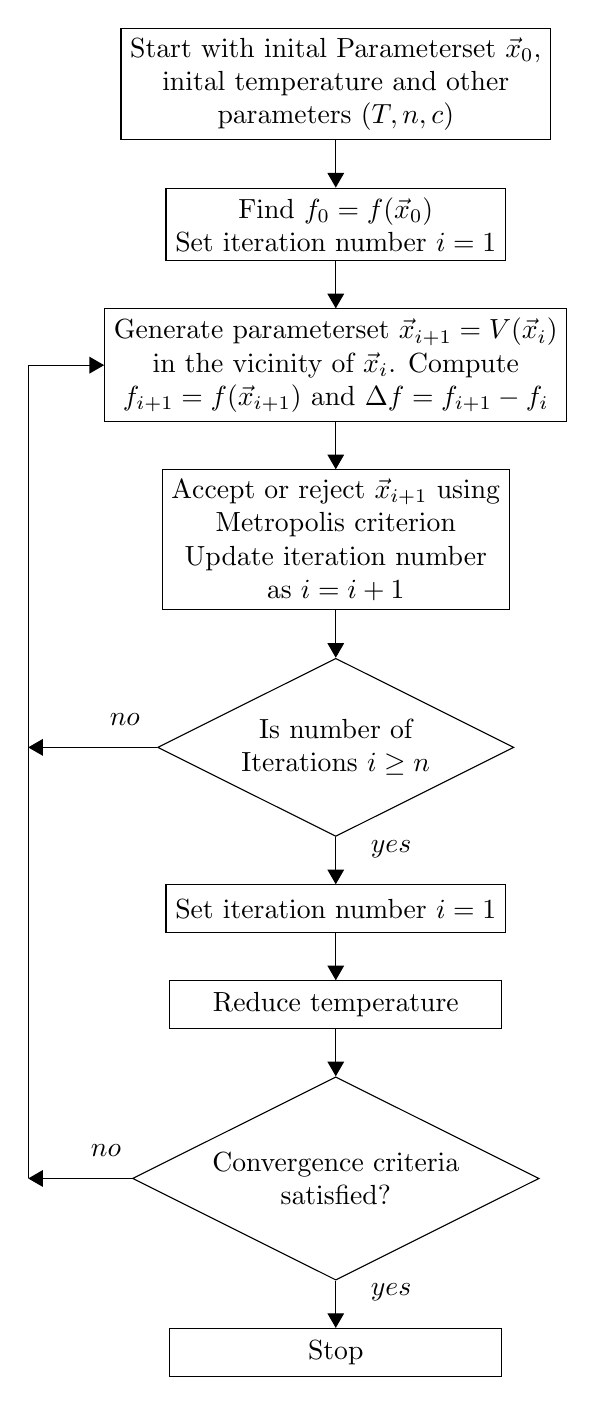
\begin{tikzpicture}[%
    >=triangle 60,              % Nice arrows; your taste may be different
    start chain=going below,    % General flow is top-to-bottom
    node distance=6mm and 60mm, % Global setup of box spacing
    every join/.style={norm},   % Default linetype for connecting boxes
    ]
% ------------------------------------------------- 
% A few box styles 
% <on chain> *and* <on grid> reduce the need for manual relative
% positioning of nodes
\tikzset{
  base/.style={draw, on chain, on grid, align=center, minimum height=4ex},
  proc/.style={base, rectangle, minimum width = 12em},
  test/.style={base, diamond, aspect=2},
  term/.style={proc, rounded corners},
  % coord node style is used for placing corners of connecting lines
  coord/.style={coordinate, on chain, on grid, node distance=6mm and 25mm},
  % nmark node style is used for coordinate debugging marks
  nmark/.style={draw, cyan, circle, font={\sffamily\bfseries}},
  % -------------------------------------------------
  % Connector line styles for different parts of the diagram
  norm/.style={->, draw, lcnorm},
  free/.style={->, draw, lcfree},
  cong/.style={->, draw, lccong},
  it/.style={font={\small\itshape}}
}
% -------------------------------------------------
% Start by placing the nodes
\node [proc] (p0) {Start with inital Parameterset $\vec{x}_0$,\\inital temperature and other\\parameters ($T,n,c$)};
% Use join to connect a node to the previous one 
\node [proc, join]      {Find $f_0=f(\vec{x}_0)$\\Set iteration number $i=1$};
\node [proc, join] (pgen) {Generate parameterset $\vec{x}_{i+1} = V(\vec{x}_i)$\\ in the vicinity of $\vec{x}_i$. Compute\\ $f_{i+1}=f(\vec{x}_{i+1})$ and $\Delta f  = f_{i+1} - f_{i}$};%

\node [proc,join] (p2) {Accept or reject $\vec{x}_{i+1}$ using\\ Metropolis criterion\\Update iteration number\\as $i=i+1$};
\node [test, join] (t2) {Is number of\\ Iterations $i\geq n$};
\node [proc, join] (pupdate){Set iteration number $i=1$};
\node [proc, join] {Reduce temperature};

\node [test, join] (tconv) {Convergence criteria\\satisfied?};
\node [proc, join] (pstop){Stop};

\node [coord, right=of pgen,  xshift=-4em] (c1)  {}; 
\node [coord, left=of t2,  xshift=-4em] (c4)  {};
\node [coord, left=of tconv,  xshift=-4em] (cnoconv)  {}; 
\node [coord, left=of pgen,  xshift=-4em] (cgen)  {}; 

\path (tconv.south) to node [near start, xshift=2em] {$yes$} (pstop);
\path (t2.south) to node [near start, xshift=2em] {$yes$} (pupdate);

\path (t2.west) to node [near start, yshift=1em] {$no$} (c4);
  \draw [->] (t2.west) -- (c4);

\path (tconv.west) to node [near start, yshift=1em] {$no$} (cnoconv);
  \draw [->] (tconv.west) -- (cnoconv);
\draw [->] (cnoconv) -- (cgen) -- (pgen.west);


\end{tikzpicture}
\caption{Diagrammablauf des Simulated Annealing Algorithmus nach Singiresu S. Rao: Engineering Optimization: Theory and Practice}
\label{simanFlowChart}
\end{figure}
\clearpage
%\subsection{Beispiel}

%Von der Funktion $f(x) = \frac{4-x-1.3*sin(2*(5-x)*\frac{180}{\pi})}{4-x}$ soll das Minimum zwischen 0 und 6 gefunden werden.

%\begin{description}
%\item [Step 1:] 
%\end{description}

\section{Erweiterungen}
Der Simulated Annealing Algorithmus ist die Grundlage
mehrerer Algorithmen. Der bekannteste darunter d"urfte der
Toleranzschwellen-Algorithmus sein.

W"ahrend beim Simulated Annealing eine ung"unstige
Parameterkombination mit einer gewissen Wahrscheinlichkeit und
eine bessere Parameterkombination immer akzeptiert wird, wird beim
Toleranzschwellen-Verfahren (Treshholding Accept) jede Konfiguration
akzeptiert, bei der die "Anderung unterhalb eines Schwellenwertes
liegt. Das heisst eine akzeptierte Kombination muss entweder besser
sein als die Alte, oder darf maximal bis zu einem bestimmten Schwellwert
"uber der alten Kombination liegen. Dadurch entf"allt die Abfrage ob die
neue Kombination besser ist als die alte, da die Differenz $\Delta f$
immer unter der Toleranzschwelle liegen muss.

Es konnte in verschiedenen Versuchsreihen gezeigt werden, dass das
Toleranz\-schwellen-Verfahren meist bessere L"osungen errechnet als das
Simulated Annealing und gleichzeitig weniger Zeit ben"otigt.

\section{Sourcefiles}
\begin{description}
	\item [Code:] \url{https://github.com/RGassmann/Simulated-Annealing}
	\item [Video:] \url{http://www.youtube.com/watch?v=iaq_Fpr4KZc}
\end{description}
